\section{Реализация набора динамических библиотек, подключаемых к задачнику Unix Taskbook}

\begin{figure}[htbp]%
    \centering
    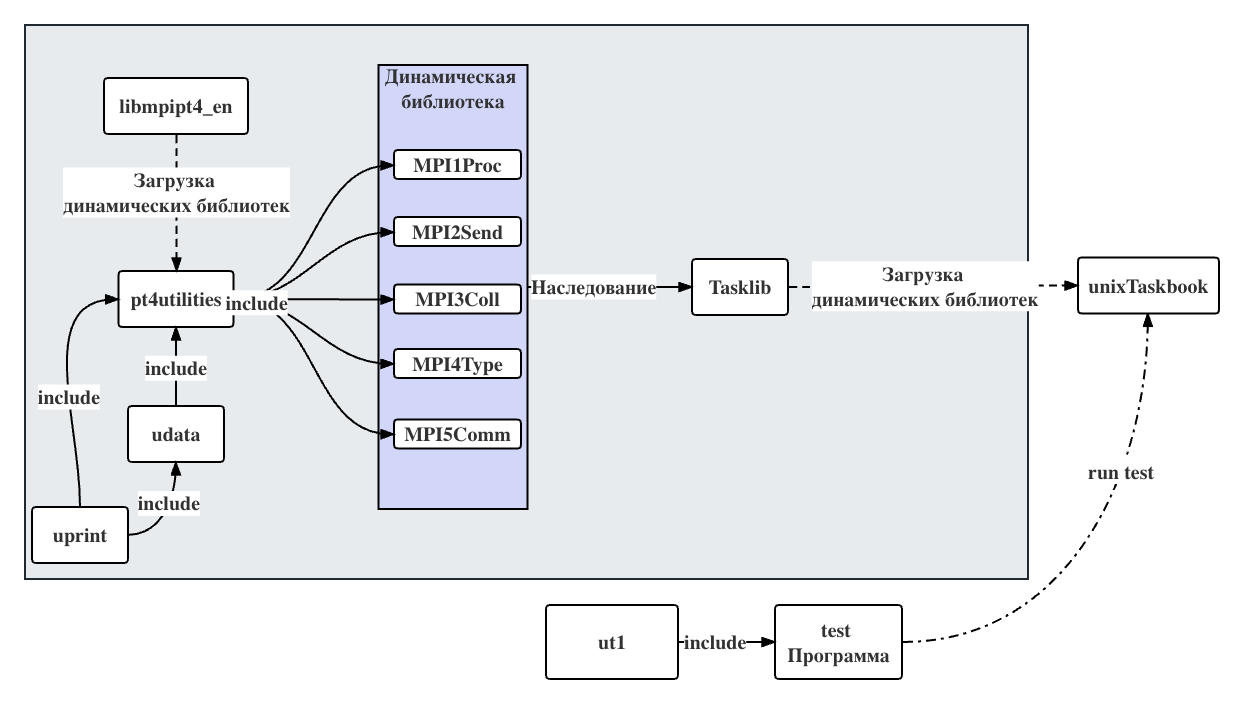
\includegraphics[width=1\linewidth]{images/relation.png}%子图文件名
    \caption{Отношения между динамическими библиотеками и компонентами.}%总标题
    \label{relation}%总标签
\end{figure}

\subsection{Проектные решения для динамических библиотек}
Учитывая различия между разными группами задач, например, они могут иметь разные методы компиляции, параметры 
компиляции, количество задач и т.д., для совместимости с разными группами задач нам необходимо разработать 
интерфейс для регулирования различных реализаций динамических библиотек. То есть, все эти динамические библиотеки 
будут реализовывать этот интерфейс, поэтому все динамические библиотеки будут иметь некоторые общие поля или 
методы, но эти поля и методы могут иметь различные значения или реализации.

\subsubsection{Интерфейс TaskLib}

\lstset{language=c++}
\begin{lstlisting}
#ifndef TASKLIB_HPP
#define TASKLIB_HPP

#include "header.hpp"

class TaskLib
{
protected:
	std::vector<std::string> task_text_russian;
	std::vector<std::string> task_text_chinese;
	std::vector<std::string> task_text_english;

	std::vector<std::string> compile_argv;

	std::vector<std::string> execute_argv;

	std::vector<std::string> test_files;
	std::string control_file = "_control.tst";
	std::string result_file;

	std::string compiler;

	std::string library_name;

	int task_count;
	int output = 1;
	int f_control;
	int total_test_count;

public:
	bool print_file = true;		  
	bool print_task_info = false; 
	// Public real function
	// Implemented by tasklib itself
	TaskLib() {}
	int get_task_count() const;
	std::vector<std::string> get_execute_argv() const;
	std::string get_task_info(int task_num, int language_option) const;
	// The virtual function (interface)
	// Implemented by each tasklib itself
	virtual void utb_print_task_info(int task_num, int language_option) {} 
	virtual void utb_generate_task_test(int task_num, int test_num) = 0;   
	virtual void utb_generate_task_control(int task_num) = 0;
	virtual void utb_print_extra_info(int task_num) = 0;
	virtual int utb_check_program(int test_num) const = 0;
	virtual ~TaskLib() {}

	// friend class
	friend class UnixTaskbook;
};

// the types of the class factories
typedef TaskLib *create_t();
typedef void destroy_t(TaskLib *);

#endif
\end{lstlisting}

Данный заголовочный файл TaskLib.hpp содержит объявление класса TaskLib, который 
является базовым классом для библиотек задач. Класс TaskLib содержит ряд защищенных 
полей, таких как векторы для хранения тестов, аргументов компиляции и исполнения 
программы, а также строк для имени файла управления и результата. Также есть строка 
для хранения имени компилятора и счетчики задач и тестов.

Класс TaskLib определяет несколько чисто виртуальных функций, которые 
должны быть реализованы в производных классах библиотек задач. Эти 
функции позволяют выводить информацию о задаче на разных языках, генерировать 
тесты и файлы управления, проверять ответы программы на тестах и выводить дополнительную 
информацию о задаче.

Таким образом, класс TaskLib является основой для создания библиотек разных 
задач на программирования и предоставляет удобный интерфейс для работы с задачами.

Класс TaskLib содержит защищенные поля:

\begin{itemize}
\item \textbf{std::vectorstd::string task\_text\_russian} - вектор строк, содержащий текст задач на русском языке;
\item \textbf{std::vectorstd::string task\_text\_chinese} - вектор строк, содержащий текст задач на китайском языке;
\item \textbf{std::vectorstd::string task\_text\_english} - вектор строк, содержащий текст задач на английском языке;
\item \textbf{std::vectorstd::string compile\_argv} - вектор строк, содержащий аргументы компиляции программы;
\item \textbf{std::vectorstd::string execute\_argv} - вектор строк, содержащий аргументы исполнения программы;
\item \textbf{std::vectorstd::string test\_files} - вектор строк, содержащий имена файлов с тестами;
\item \textbf{std::string control\_file} - строка, содержащая имя файла управления;
\item \textbf{std::string result\_file} - строка, содержащая имя файла с результатами;
\item \textbf{std::string compiler} - строка, содержащая имя компилятора;
\item \textbf{std::string library\_name} - строка, содержащая имя библиотеки задач;
\item \textbf{int task\_count} - целое число, содержащее количество задач в библиотеке;
\item \textbf{int output} - целое число, определяющее формат вывода результатов;
\item \textbf{int f\_control} - целое число, определяющее формат файла управления;
\item \textbf{int total\_test\_count} - целое число, содержащее общее количество тестов для всех задач в библиотеке.
\end{itemize}

Класс TaskLib определяет несколько методов:

\begin{itemize}
\item \textbf{TaskLib()} - конструктор класса;
\item \textbf{int get\_task\_count() const} - метод, возвращающий количество задач в библиотеке;
\item \textbf{std::vectorstd::string get\_execute\_argv() const} - метод, возвращающий вектор аргументов исполнения программы;
\item \textbf{std::string get\_task\_info(int task\_num, int language\_option) const} - метод, возвращающий текст задачи на определенном языке;
\item \textbf{virtual void utb\_print\_task\_info(int task\_num, int language\_option)} - чисто виртуальный метод, выводящий информацию о задаче на определенном языке;
\item \textbf{virtual void utb\_generate\_task\_test(int task\_num, int test\_num) = 0} - чисто виртуальный метод, генерирующий тест для задачи;
\item \textbf{virtual void utb\_generate\_task\_control(int task\_num) = 0} - чисто виртуальный метод, генерирующий файл управления для задачи;
\item \textbf{virtual void utb\_print\_extra\_info(int task\_num) = 0} - чисто виртуальный метод, выводящий дополнительную информацию о задаче;
\item \textbf{virtual int utb\_check\_program(int test\_num) const = 0} - Чисто виртуальный метод для проверки правильности результата выполнения задачи программирования;
\item \textbf{virtual $\sim$TaskLib()} - виртуальный деструктор, который должен быть реализован в подклассах;
\end{itemize}

Этот файл также определяет два типа фабрик классов: create\_t и destroy\_t, которые
используются для создания и уничтожения экземпляров TaskLib.

Наконец, также объявляет класс UnixTaskbook как друга, что означает, что он имеет доступ к 
защищенным членам этого класса. Вероятно, это сделано для того, чтобы класс UnixTaskbook мог 
управлять задачами, реализованными в классе TaskLib, и использовать его функциональность в 
своих собственных целях. Фактически, Unix Taskbook, как ядро, используется для управления всем процессом, включая создание и управление тестовыми сценариями, которые проверяют реализацию задач в TaskLib.

\lstset{language=c++}
\begin{lstlisting}
#include "tasklib.hpp"

int TaskLib::get_task_count() const
{
	return task_count;
}
std::vector<std::string> TaskLib::get_execute_argv() const
{
	return execute_argv;
}

std::string TaskLib::get_task_info(int task_num, int language_option) const
{
	switch (language_option)
	{
	case 0:
		return task_text_russian[task_num - 1];
	case 1:
		return task_text_chinese[task_num - 1];
	case 2:
		return task_text_english[task_num - 1];
	default:
		return task_text_russian[task_num - 1];
	}
}
\end{lstlisting}

Класс TaskLib реализует несколько методов, которые позволяют получить информацию о задачах и их количестве.

Метод "get\_task\_count" возвращает количество задач в объекте TaskLib.

Метод "get\_execute\_argv" возвращает вектор строк, содержащих аргументы командной строки для компиляции и запуска программы.

Метод "get\_task\_info" возвращает строку с текстом задачи на заданном языке. Номер задачи и язык задаются в аргументах метода. Если заданный язык не поддерживается, метод вернет текст задачи на русском языке.

Все методы класса TaskLib объявлены как константные, что означает, что они не изменяют состояние объекта TaskLib.

Защищенные члены класса TaskLib могут быть использованы только внутри класса или его наследников, а публичные методы могут быть вызваны извне.

Методы класса TaskLib являются важными для управления задачами в рамках Unix Taskbook.

\subsubsection{Особенности динамической библиотеки параллельного программирования MPI}

Для большинства задач в группе задач по программированию мы просто компилируем тестируемый файл с помощью gcc/g++ для создания 
исполняемого файла <имя\_файла>.out и затем выполняем его с помощью . /<имя\_файла>.out, чтобы выполнить его непосредственно из командной строки.

Но в группах параллельных программ мы необходимо использовать реализацию MPI, называемую MPICH
\footnote{MPICH является высокопроизводительной и широко переносимой реализацией 
стандарта MPI, который представляет собой интерфейс передачи сообщений для распределенных 
приложений, использующих параллельные вычисления. MPICH и его производные формируют самые 
широко используемые реализации MPI в мире. 

MPICH поддерживает последнюю версию стандарта MPI-2 и может быть установлен и запущен
 на платформах Windows и UNIX. MPICH предоставляет компоненты, среды выполнения и 
 инструменты, необходимые для компиляции и запуска программ MPI \cite{ref3} \cite{ref5}. 
 MPICH также обладает рядом преимуществ, таких как оптимизация коллективных операций 
 связи \cite{ref4}, эффективная поддержка многопоточной связи MPI  и совместимость с 
 другими реализациями MPI.}, для выполнения параллельных вычислительных задач. 

В этом случае, если мы используем gcc для компиляции тестового файла, нам придется 
вручную добавлять опции компилятора и компоновщика, связанные с MPI, что, конечно, 
обременительно, поэтому для классов, относящихся к группе задач параллельного 
программирования, нам нужно наследовать класс TaskLib и установить поле \textbf{compiler} в "mpicc"
\footnote{mpicc является оберткой над базовым компилятором C, которая автоматически 
добавляет необходимые опции компилятора и линковщика для MPI-программ. Использование
 mpicc упрощает компиляцию и сборку MPI-программ, без необходимости указывать 
 расположение заголовочных и библиотечных файлов MPI \cite{ref7} \cite{ref8}. 
 mpicc является инструментом, предоставляемым реализацией MPI (например, 
 MPICH или Open MPI), который может адаптироваться к различным реализациям 
 MPI и платформам \cite{ref9} \cite{ref10}.}.

 Для компиляции файла на языке C с помощью mpicc необходимо указать следующие параметры:

\begin{itemize}
	\item <имя\_файла>.c - задает имя или путь исходного файла на языке C;
	\item -o <имя\_файла> - задает имя или путь исполняемого файла, который будет создан при компиляции;
	\item -c - задает режим компиляции без сборки;
\end{itemize}

 
 Например, следующая команда компилирует файл MPI1Proc7.c и создает исполняемый файл MPI1Proc7.out:
 
 \centerline{\textbf{mpicc MPI1Proc7.c -o MPI1Proc7.out}}

При тестировании задачи в группах параллельных программ мы используем утилиту mpiexec 
для запуска программы. mpiexec является универсальной утилитой для запуска 
MPI-приложений, которая поддерживает различные реализации MPI и различные среды выполнения \cite{ref6}.

Для запуска MPI-приложения с помощью mpiexec необходимо указать следующие параметры:

\begin{itemize}
	\item -np <число> - задает количество MPI-процессов для запуска;
	\item -f <имя\_файла> ;
\end{itemize}

Например, следующая команда запускает MPI1Proc7.out на 8 MPI-процессах:

\centerline{\textbf{mpiexec -np 8 ./MPI1Proc7.out}} 

Таким образом, чтобы реализовать динамическую библиотеку для групп задач параллельного 
программирования, мы должны наследовать TaskLib и указать поле \textbf{executor} как "mpiexec".

\subsection{Реализованные динамические библиотеки}

Для реализации динамической библиотеки для групп задач параллельного программирования
 необходимо написать файлы классов, соответствующие каждой группе задач, и эти 
 классы, являющиеся подклассами класса TaskLib, реализуют интерфейсы, объявленные классом TaskLib.

 В дополнение к этому, поскольку мы подключаем существующую группу задач из задачника Programming Taskbook 
 в Unix Taskbook, нам также необходимо реализовать инструментальную 
 библиотеку, pt4utilities, для подключения к существующей группе задач, так что динамическая 
 библиотека, которую мы реализуем, фактически действует как промежуточное программное обеспечение, 
 передавая управление генерацией информации о задаче, представлением информации о задаче и 
 проверкой файла результатов существующей группе задач.

 Далее мы опишем интерфейсы, предоставляемые pt4utilities для динамических библиотек.

\lstset{language=c++}
\begin{lstlisting}
#ifndef PT4UTILITIES_HPP
#define PT4UTILITIES_HPP
#include <string>

typedef void __attribute__((stdcall)) (*TInitGroup)(const char *);
typedef void __attribute__((stdcall)) (*TInitTask)(int, int);

void pt4_print_task_info(std::string task_group, int task_num, int language_option);
void pt4_generate_task_test(std::string task_group, int task_num, int test_num);
void pt4_print_extra_info(std::string task_group, int task_num);
int pt4_check_program(std::string task_group, int test_num);
int pt4_mpi_get_size();

#endif
\end{lstlisting}

pt4utilities содержит объявления для всех функций, необходимых для работы с группами 
задач в задачнике Programming Taskbook.

\begin{itemize}
	\item \textbf{void pt4\_print\_task\_info(std::string task\_group, int task\_num, int language\_option)} - выводит информацию о задаче, включая ее название, описание и примеры входных и выходных данных;
	\item \textbf{void pt4\_generate\_task\_test(std::string task\_group, int task\_num, int test\_num)} - генерирует тестовые данные для задачи;
	\item \textbf{void pt4\_print\_extra\_info(std::string task\_group, int task\_num)} - выводит информацию о результатах выполнения текущего задания;
	\item \textbf{int pt4\_check\_program(std::string task\_group, int test\_num)} - проверяет программу на соответствие ожидаемому результату для заданного теста;
	\item \textbf{int pt4\_mpi\_get\_size()} - Возвращает количество процессов, необходимых для выполнения текущего тестового задания;
\end{itemize}

Вышеуказанные функции будут доступны для всех динамических библиотек, которым необходим 
доступ к уже существующим группам задач задачника Programming Taskbook, чтобы обеспечить 
управление этими группами задач.

Имея pt4utilities в качестве необходимого условия, мы можем приступить к разработке динамических библиотек.

\subsubsection{MPI1Proc}

\lstset{language=c++}
\begin{lstlisting}
#include "tasklib.hpp"
#include "pt4utilities.hpp"

class utbMPI1Proc : public TaskLib
{
private:
	std::string task_group;

public:
	utbMPI1Proc();
	virtual ~utbMPI1Proc() {}

	virtual void utb_print_task_info(int task_num, int language_option)
	{
		pt4_print_task_info(task_group, task_num, language_option);
	}

	virtual void utb_generate_task_test(int task_num, int test_num)
	{
		pt4_generate_task_test(task_group, task_num, test_num);
	}

	virtual void utb_generate_task_control(int task_num) {}

	virtual void utb_print_extra_info(int task_num)
	{
		pt4_print_extra_info(task_group, task_num);
	}

	virtual int utb_check_program(int test_num) const
	{
		return pt4_check_program(task_group, test_num);
	}

	// friend class
	friend class UnixTaskbook;
};

extern "C" TaskLib *create()
{
	return new utbMPI1Proc;
}

extern "C" void destroy(TaskLib *t)
{
	delete t;
}

utbMPI1Proc::utbMPI1Proc()
{
#if defined __linux__
	library_name = "libutbMPI1Proc.so";
#elif defined __APPLE__
	library_name = "libutbMPI1Proc.dylib";
#endif

	compiler = "mpicc";
	compile_argv = {compiler, "-Wall", "-w", "", "ut1.c", "-o"};

	execute_argv = {"mpiexec", "-np", std::to_string(pt4_mpi_get_size())};

	task_group = "MPI1Proc";
	task_count = 10;
	total_test_count = 3;

	print_file = false;
	print_task_info = true;
}

\end{lstlisting}

Задачи этой группы\cite{ref11} по MPI предназначены для тестирования умений студентов работать с параллельными вычислениями, а также для проверки их знаний по работе с входными и выходными данными в MPI. Кроме того, задачи требуют от студентов умения работать с функциями ввода-вывода и отладочными функциями в MPI.

В задачах используются различные функции MPI, такие как MPI\_Comm\_rank, MPI\_Comm\_size, MPI\_Send и MPI\_Recv. Задачи покрывают различные аспекты параллельных вычислений, такие как ввод и вывод данных, вычисления в зависимости от номера процесса и обмен данными между процессами.

Решение этих задач требует от студентов умения анализировать поставленную задачу и правильно применять соответствующие функции MPI. Это также требует от них умения работать с различными типами данных и умения разрабатывать эффективные алгоритмы для параллельных вычислений.
\subsubsection{MPI2Send}

\lstset{language=c++}
\begin{lstlisting}
#include "tasklib.hpp"
#include "pt4utilities.hpp"

class utbMPI2Send : public TaskLib
{
private:
	std::string task_group;

public:
	utbMPI2Send();
	virtual ~utbMPI2Send() {}

	virtual void utb_print_task_info(int task_num, int language_option)
	{
		pt4_print_task_info(task_group, task_num, language_option);
	}

	virtual void utb_generate_task_test(int task_num, int test_num)
	{
		pt4_generate_task_test(task_group, task_num, test_num);
	}

	virtual void utb_generate_task_control(int task_num) {}

	virtual void utb_print_extra_info(int task_num)
	{
		pt4_print_extra_info(task_group, task_num);
	}

	virtual int utb_check_program(int test_num) const
	{
		return pt4_check_program(task_group, test_num);
	}

	// friend class
	friend class UnixTaskbook;
};

extern "C" TaskLib *create()
{
	return new utbMPI2Send;
}

extern "C" void destroy(TaskLib *t)
{
	delete t;
}

utbMPI2Send::utbMPI2Send()
{
#if defined __linux__
	library_name = "libutbMPI2Send.so";
#elif defined __APPLE__
	library_name = "libutbMPI2Send.dylib";
#endif

	compiler = "mpicc";
	compile_argv = {compiler, "-Wall", "-w", "", "ut1.c", "-o"};

	execute_argv = {"mpiexec", "-np", std::to_string(pt4_mpi_get_size())};

	task_group = "MPI2Send";
	task_count = 32;
	total_test_count = 3;

	print_file = false;
	print_task_info = true;
}

\end{lstlisting}

Задачи этой группы\cite{ref12} в основном связаны с коммуникацией с MPI (Message Passing Interface). 
Эти задачи включают отправку и получение данных с помощью MPI, как блокирующие, так 
и неблокирующие коммуникации, и проверяют навыки студентов в области программирования 
и параллельных вычислений. Задачи по блокирующей коммуникации проверяют знания 
студентов об использовании основных функций, таких как MPI\_Send и MPI\_Recv, а также 
о том, как выполнять операции сортировки и кэширования данных. Задачи по неблокирующей 
коммуникации проверяют, как студенты используют такие функции, как MPI\_Issend, 
MPI\_Wait, MPI\_Recv и MPI\_Test для асинхронной коммуникации и как справляться с 
проблемами отладки, которые могут возникнуть при параллельных вычислениях.

\subsubsection{MPI3Coll}

\lstset{language=c++}
\begin{lstlisting}
#include "tasklib.hpp"
#include "pt4utilities.hpp"

class utbMPI3Coll : public TaskLib
{
private:
	std::string task_group;

public:
	utbMPI3Coll();
	virtual ~utbMPI3Coll() {}

	virtual void utb_print_task_info(int task_num, int language_option)
	{
		pt4_print_task_info(task_group, task_num, language_option);
	}

	virtual void utb_generate_task_test(int task_num, int test_num)
	{
		pt4_generate_task_test(task_group, task_num, test_num);
	}

	virtual void utb_generate_task_control(int task_num) {}

	virtual void utb_print_extra_info(int task_num)
	{
		pt4_print_extra_info(task_group, task_num);
	}

	virtual int utb_check_program(int test_num) const
	{
		return pt4_check_program(task_group, test_num);
	}

	// friend class
	friend class UnixTaskbook;
};

extern "C" TaskLib *create()
{
	return new utbMPI3Coll;
}

extern "C" void destroy(TaskLib *t)
{
	delete t;
}

utbMPI3Coll::utbMPI3Coll()
{
#if defined __linux__
	library_name = "libutbMPI3Coll.so";
#elif defined __APPLE__
	library_name = "libutbMPI3Coll.dylib";
#endif

	compiler = "mpicc";
	compile_argv = {compiler, "-Wall", "-w", "", "ut1.c", "-o"};

	execute_argv = {"mpiexec", "-np", std::to_string(pt4_mpi_get_size())};

	task_group = "MPI3Coll";
	task_count = 28;
	total_test_count = 3;

	print_file = false;
	print_task_info = true;
}
\end{lstlisting}

Задачи этой группы\cite{ref13} относятся к параллельному программированию с использованием 
библиотеки MPI (Message Passing Interface) для обмена данными между процессами. В 
каждом вопросе ученику предлагается написать программу на языке программирования, 
которая выполняет определенную задачу с помощью функций MPI.

Задачи проверяют знание основных функций MPI для передачи данных между 
процессами, таких как MPI\_Bcast, MPI\_Gather, MPI\_Scatter, MPI\_Reduce и 
MPI\_Allreduce, а также способность к решению задач по передаче данных и 
совместной обработке данных между процессами. Решение этих задач помогает 
ученикам улучшить навыки в области параллельного программирования, такие как 
эффективное использование ресурсов, разбиение задач на небольшие подзадачи, передача 
данных между процессами и совместная обработка данных.

\subsubsection{MPI4Type}

\lstset{language=c++}
\begin{lstlisting}
#include "tasklib.hpp"
#include "pt4utilities.hpp"

class utbMPI4Type : public TaskLib
{
private:
	std::string task_group;

public:
	utbMPI4Type();
	virtual ~utbMPI4Type() {}

	virtual void utb_print_task_info(int task_num, int language_option)
	{
		pt4_print_task_info(task_group, task_num, language_option);
	}

	virtual void utb_generate_task_test(int task_num, int test_num)
	{
		pt4_generate_task_test(task_group, task_num, test_num);
	}

	virtual void utb_generate_task_control(int task_num) {}

	virtual void utb_print_extra_info(int task_num)
	{
		pt4_print_extra_info(task_group, task_num);
	}

	virtual int utb_check_program(int test_num) const
	{
		return pt4_check_program(task_group, test_num);
	}

	// friend class
	friend class UnixTaskbook;
};

extern "C" TaskLib *create()
{
	return new utbMPI4Type;
}

extern "C" void destroy(TaskLib *t)
{
	delete t;
}

utbMPI4Type::utbMPI4Type()
{
#if defined __linux__
	library_name = "libutbMPI4Type.so";
#elif defined __APPLE__
	library_name = "libutbMPI4Type.dylib";
#endif

	compiler = "mpicc";
	compile_argv = {compiler, "-Wall", "-w", "", "ut1.c", "-o"};

	execute_argv = {"mpiexec", "-np", std::to_string(pt4_mpi_get_size())};

	task_group = "MPI4Type";
	task_count = 22;
	total_test_count = 3;

	print_file = false;
	print_task_info = true;
}
\end{lstlisting}

Задачи этой группы\cite{ref14} относятся к параллельному программированию 
с использованием MPI (Message Passing Interface), протокола для 
обмена сообщениями между процессами, работающими на разных узлах 
вычислительного кластера. Задачи касаются создания и использования 
производных типов данных и упаковки данных для передачи между процессами.

Ученик проверяет свои знания по работе с MPI и способности 
создавать производные типы данных и эффективно упаковывать 
данные для передачи между процессами. Также ученик улучшает 
свои навыки работы с функциями MPI\_Send, MPI\_Recv, MPI\_Pack и 
MPI\_Unpack, а также создания новых типов данных с помощью 
функций MPI\_Type\_create\_resized и MPI\_Type\_struct. Кроме того, 
ученик практикует работу с коллективными операциями MPI.

\subsubsection{MPI5Comm}

\lstset{language=c++}
\begin{lstlisting}
#include "tasklib.hpp"
#include "pt4utilities.hpp"

class utbMPI5Comm : public TaskLib
{
private:
	std::string task_group;

public:
	utbMPI5Comm();
	virtual ~utbMPI5Comm() {}

	virtual void utb_print_task_info(int task_num, int language_option)
	{
		pt4_print_task_info(task_group, task_num, language_option);
	}

	virtual void utb_generate_task_test(int task_num, int test_num)
	{
		pt4_generate_task_test(task_group, task_num, test_num);
	}

	virtual void utb_generate_task_control(int task_num) {}

	virtual void utb_print_extra_info(int task_num)
	{
		pt4_print_extra_info(task_group, task_num);
	}

	virtual int utb_check_program(int test_num) const
	{
		return pt4_check_program(task_group, test_num);
	}

	// friend class
	friend class UnixTaskbook;
};

extern "C" TaskLib *create()
{
	return new utbMPI5Comm;
}

extern "C" void destroy(TaskLib *t)
{
	delete t;
}

utbMPI5Comm::utbMPI5Comm()
{
#if defined __linux__
	library_name = "libutbMPI5Comm.so";
#elif defined __APPLE__
	library_name = "libutbMPI5Comm.dylib";
#endif

	compiler = "mpicc";
	compile_argv = {compiler, "-Wall", "-w", "", "ut1.c", "-o"};

	execute_argv = {"mpiexec", "-np", std::to_string(pt4_mpi_get_size())};

	task_group = "MPI5Comm";
	task_count = 32;
	total_test_count = 3;

	print_file = false;
	print_task_info = true;
}
\end{lstlisting}

В задачах этой группы\cite{ref15} речь идет о программировании с использованием 
MPI (Message Passing Interface), который является стандартом для
 взаимодействия параллельных программ. Основной целью всех задач 
 является создание новых коммуникаторов и/или виртуальных топологий для
  обеспечения эффективного взаимодействия между процессами.

В задачах проверяются знания студента по использованию функций 
MPI\_Comm\_group, MPI\_Group\_incl, MPI\_Group\_excl, MPI\_Comm\_create,
 MPI\_Comm\_split, MPI\_Cart\_create, MPI\_Cart\_coords, MPI\_Cart\_sub, 
 MPI\_Graph\_create, MPI\_Dist\_graph\_create, а также навыки по работе
  с коллективными операциями (например, MPI\_Bcast, MPI\_Reduce), обмену
   сообщениями между процессами, созданию новых коммуникаторов и 
   виртуальных топологий. В разных задачах ученик должен будет решать
    разные задачи, например, отправлять и получать числа, находить 
	минимальное значение, определять координаты процесса в топологии, 
	отправлять данные из процессов в строке/столбце топологии и т.д.


\newpage
